\documentclass[../Main.tex]{subfiles}

\begin{document}

\thispagestyle{empty} % suppress header

\addcontentsline{toc}{section}{Historias de usuario}
\subsection*{Historias de usuario}
\begin{justify}
El documento adjunto se encuentra en la carpeta Diseño como:
\begin{itemize}
    \item \texttt{historias\_de\_usuario\_GQuestions\_TG.pdf}
\end{itemize}
\end{justify}

    \begin{table}[H]
	\begin{Center}
		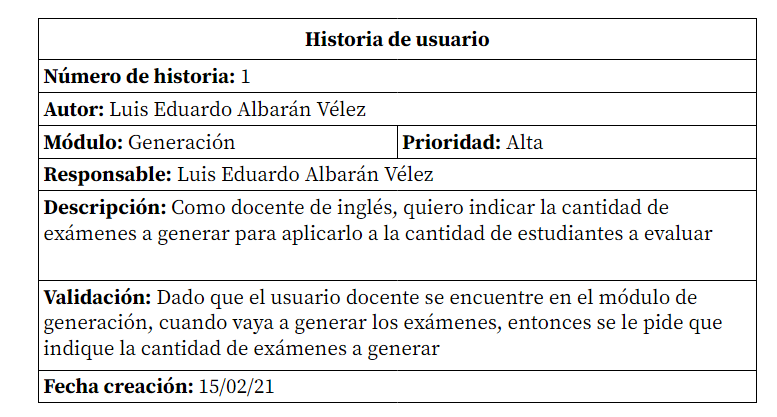
\includegraphics[width=4.8in,height=2.6in]{./images/hu_1}
	    \caption{Historia de usuario 1}
	    Fuente: Elaboración propia
        \label{tab:section}
	\end{Center}
    \end{table}

    \begin{table}[H]
	\begin{Center}
		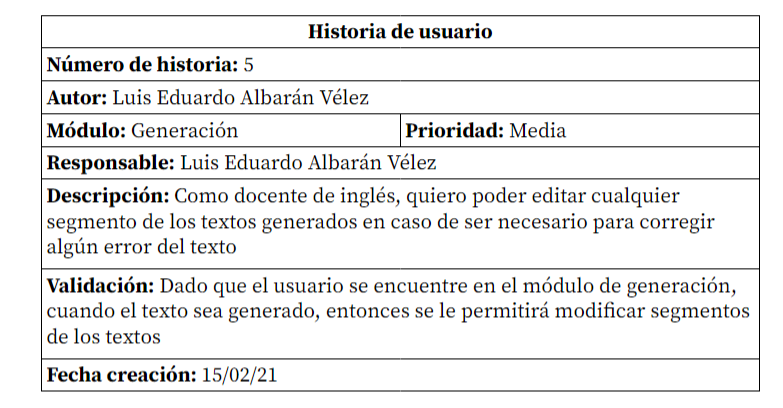
\includegraphics[width=4.7in,height=2.5in]{./images/hu_5}
	    \caption{Historia de usuario 5}
	    Fuente: Elaboración propia
        \label{tab:section}
	\end{Center}
    \end{table}
  
\newpage   
\thispagestyle{empty} % suppress header  
        \begin{table}[H]
	\begin{Center}
		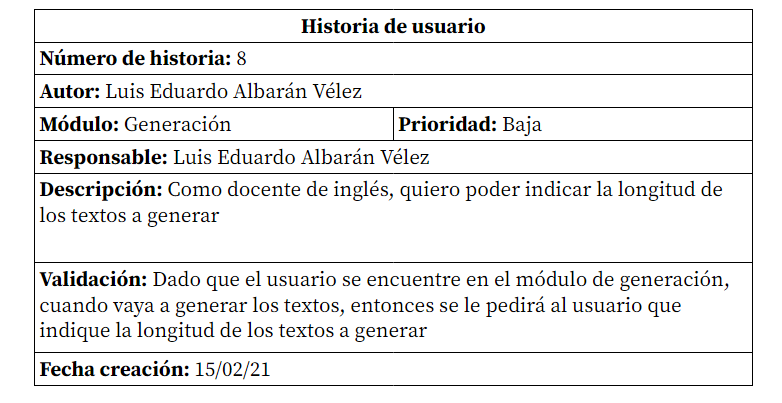
\includegraphics[width=4.8in,height=2.5in]{./images/hu_8}
	    \caption{Historia de usuario 8}
	    Fuente: Elaboración propia
        \label{tab:section}
	\end{Center}
    \end{table}


        \begin{table}[H]
	\begin{Center}
		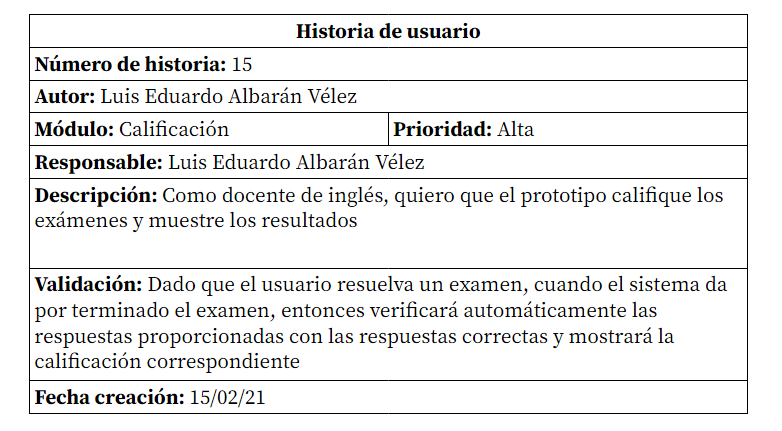
\includegraphics[width=4.8in,height=2.7in]{./images/hu_15}
	    \caption{Historia de usuario 15}
	    Fuente: Elaboración propia
        \label{tab:section}
	\end{Center}
    \end{table}
\addcontentsline{toc}{section}{Justificación selección de algoritmos}
\subsection*{Justificación selección de algoritmos}
\begin{justify}
El documento adjunto se encuentra en la carpeta raíz como:
\begin{itemize}
    \item \texttt{justificacion\_seleccion\_algoritmos\_GQuestions\_TG.pdf}
\end{itemize}
\addcontentsline{toc}{section}{Documentos recolectados}
\subsection*{Documentos recolectados}
El documento adjunto se encuentra en la carpeta raíz como:
\begin{itemize}
    \item \texttt{tabla\_documentos\_recolectados.pdf}
\end{itemize}
\end{justify}

\begin{justify}
\addcontentsline{toc}{section}{Algoritmos recolectados}
\subsection*{Algoritmos recolectados}
El documento adjunto se encuentra en la carpeta raíz como:
\begin{itemize}
    \item \texttt{tabla\_algoritmos\_recolectados.pdf}
\end{itemize}
\end{justify}

\addcontentsline{toc}{section}{Prototipo de interfaz GQuestions}
\subsection*{Prototipo de interfaz GQuestions}
\begin{justify}
El documento adjunto se encuentra en la carpeta Diseño como:
\begin{itemize}
    \item \texttt{prototipo\_de\_interfaz\_GQuestions\_TG.pdf}
\end{itemize}
\end{justify}

\addcontentsline{toc}{section}{Manuales de usuario}
\subsection*{Manuales de usuario}
\begin{justify}
El documento adjunto se encuentra en la carpeta raíz como:
\begin{itemize}
    \item \texttt{manual\_de\_usuario\_docentes\_GQuestions.pdf}
    
    \item \texttt{manual\_de\_usuario\_estudiantes\_GQuestions.pdf}
\end{itemize}
\end{justify}

\addcontentsline{toc}{section}{Plan de pruebas}
\subsection*{Documento plan de pruebas}
\begin{justify}
El documento adjunto se encuentra en la carpeta raíz como:
\begin{itemize}
    \item \texttt{plan\_de\_pruebas\_GQuestions.pdf}
\end{itemize}
\end{justify}

\addcontentsline{toc}{section}{Encuestas}
\subsection*{Encuestas}
\begin{justify}
El documento adjunto se encuentra en la carpeta Encuestas como:
\begin{itemize}
    \item \texttt{encuesta\_1\_GQuestions\_google\_forms.pdf}
    \item \texttt{encuesta\_2\_GQuestions\_google\_forms.pdf}
    \item \texttt{encuesta\_3\_usabilidad\_docente\_GQuestions\_google\_forms.pdf}
    \item \texttt{encuesta\_3\_usabilidad\_estudiantes\_GQuestions\_google\_forms.pdf}
\end{itemize}
\end{justify}

\end{document}